%%%%%%%%%%%%%%%%%%%%%%%%%%%%%%%%%%%%

\section{最小二乗法による直線の当てはめ}

%%%%%%%%%%%%%%%%%%%%%%%%%%%%%%%%%%%%

\subsection{最良の直線を見つけるための客観的な基準}

%%%%%%%%%%%%%%%%%%%%%%%%%%%%%%%%%%%

\begin{frame}
\frametitle{最良の直線を見つけるための客観的な基準}

\begin{itemize}

\item 残差が小さい直線を求める：
\begin{enumerate}
\item 方法1：残差の絶対値の和を最小化する
\[ |e_1| + |e_2| + \cdots + |e_n| \]
\item 方法2：残差の二乗和を最小化する――\hl{最小二乗法}
\[ e_1^2 + e_2^2 + \cdots + e_n^2 \]
\end{enumerate}

\item なぜ最小二乗法か？
\begin{enumerate}
\item 最も広く使われている
\item 手計算およびソフトウェアによる計算が容易
\item 多くの場面で、2倍の大きさの残差は通常2倍以上に悪いとみなされる
\end{enumerate}

\end{itemize}

\end{frame}

%%%%%%%%%%%%%%%%%%%%%%%%%%%%%%%%%%

\begin{frame}
\frametitle{最小二乗直線}

\[ \mathhl{ \hat{y} = \beta_0 + \beta_1 x } \]

\begin{itemize}
\item $\hat{y}$：目的変数$y$の予測値
\item $\beta_0$：切片（母数）
\begin{itemize}
\item $b_0$：切片（点推定量）
\end{itemize}
\item $\beta_1$：傾き（母数）
\begin{itemize}
\item $b_1$：傾き（点推定量）
\end{itemize}
\item $x$：説明変数
\end{itemize}

\end{frame}

%%%%%%%%%%%%%%%%%%%%%%%%%%%%%%%%%%

\subsection{最小二乗直線の条件}

%%%%%%%%%%%%%%%%%%%%%%%%%%%%%%%%%%%

\begin{frame}
\frametitle{最小二乗直線の条件}

\begin{enumerate}

\item 線形性

\item 残差がほぼ正規分布に従う

\item 等分散性（一定のばらつき）

\end{enumerate}

\end{frame}

%%%%%%%%%%%%%%%%%%%%%%%%%%%%%%%%%%

\begin{frame}
\frametitle{条件（1）：線形性}

\begin{itemize}

\item 説明変数と目的変数の関係は線形でなければならない。

\item 非線形な関係へのモデル当てはめ手法も存在するが、本講義の範囲を超える。この話題に興味があれば、\href{http://www.openintro.org/download.php?file=os2_extra_nonlinear_relationships&referrer=/stat/textbook.php}{openintro.orgのオンライン補足資料}で新しい手法を学べる。

\item 散布図または\hl{残差プロット}を用いて確認する。

\end{itemize}

\begin{center}
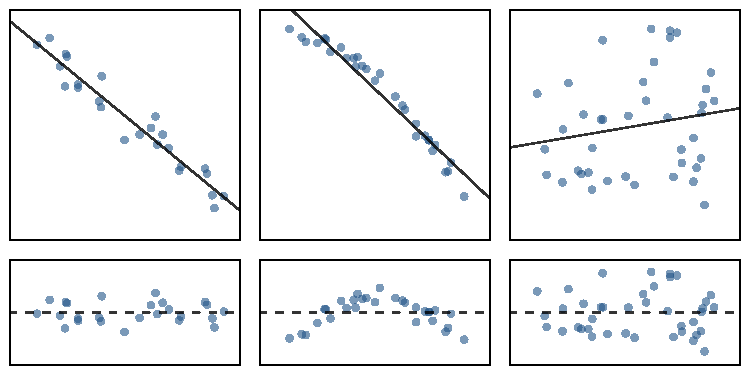
\includegraphics[width=0.7\textwidth]{8-2_least_square_reg/figures/sampleLinesAndResPlots/sampleLinesAndResPlots}
\end{center}

\end{frame}

%%%%%%%%%%%%%%%%%%%%%%%%%%%%%%%%%%

\begin{frame}[shrink=15]
\frametitle{残差プロットの見方}

\twocol{0.5}{0.5}
{
\begin{center}
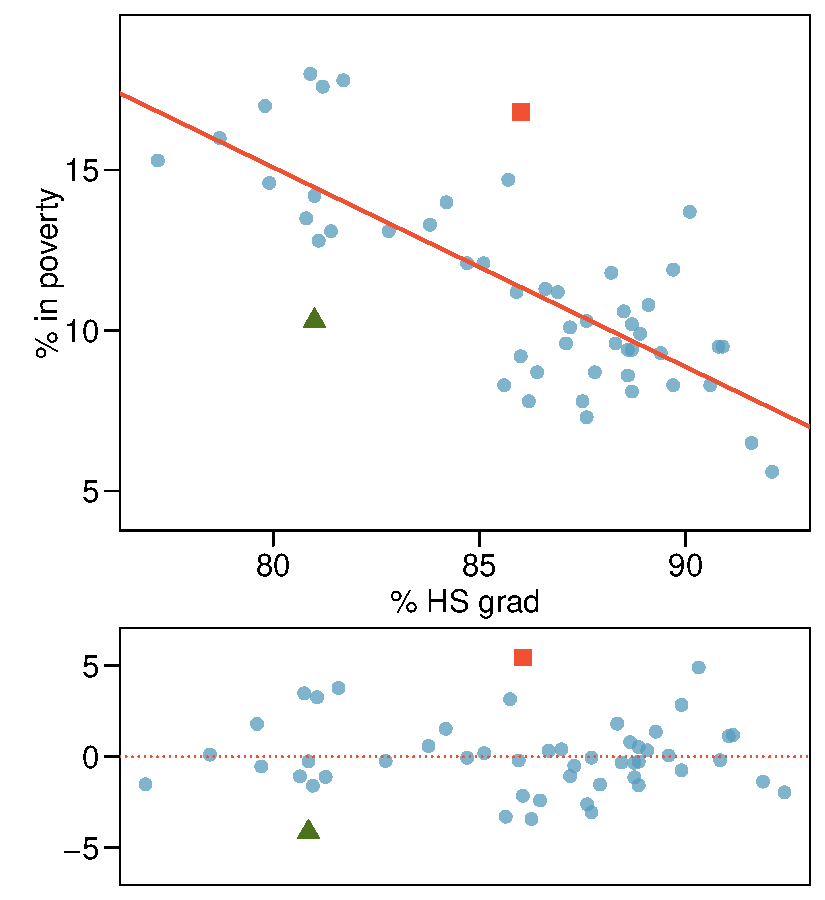
\includegraphics[width=\textwidth]{8-2_least_square_reg/figures/poverty/poverty_hsgrad_resplot}
\end{center}
}
{
{\small
\green{{\large $\blacktriangle$}} \hl{RI（ロードアイランド州）:}
\begin{align*}
\%~HS~grad &= 81,\quad \%~in~poverty = 10.3 \\
\widehat{\%~in~poverty} &= 64.68 - 0.62 \times 81 = 14.46 \\
e &= 10.3 - 14.46 = \green{$-4.16$}
\end{align*}
\textcolor{red}{{\normalsize $\blacksquare$}} \hl{DC（ワシントンDC）:}
\begin{align*}
\%~HS~grad &= 86,\quad \%~in~poverty = 16.8 \\
\widehat{\%~in~poverty} &= 64.68 - 0.62 \times 86 = 11.36 \\
e &= 16.8 - 11.36 = \textcolor{red}{5.44}
\end{align*}
}
}

\end{frame}


%%%%%%%%%%%%%%%%%%%%%%%%%%%%%%%%%%

\begin{frame}
\frametitle{条件（2）：残差がほぼ正規分布に従う}

\begin{itemize}

\item 残差はほぼ正規分布に従う必要がある。

\item データの傾向から外れた異常な観測値がある場合、この条件が満たされないことがある。

\item ヒストグラムを用いて確認する。

\end{itemize}

\begin{center}
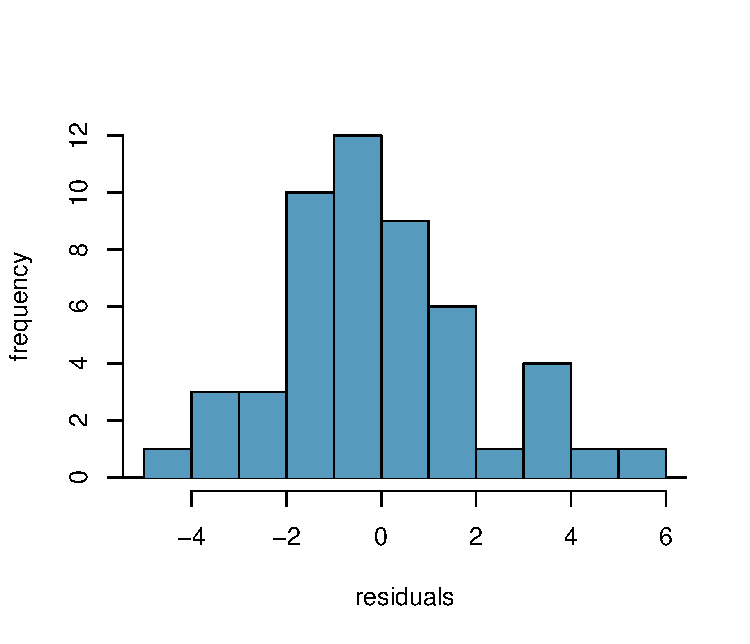
\includegraphics[width=0.5\textwidth]{8-2_least_square_reg/figures/poverty/normal_res}
\end{center}

\end{frame}

%%%%%%%%%%%%%%%%%%%%%%%%%%%%%%%%%%

\begin{frame}
\frametitle{条件（3）：等分散性（一定のばらつき）}

\twocol{0.5}{0.5}
{
\begin{center}
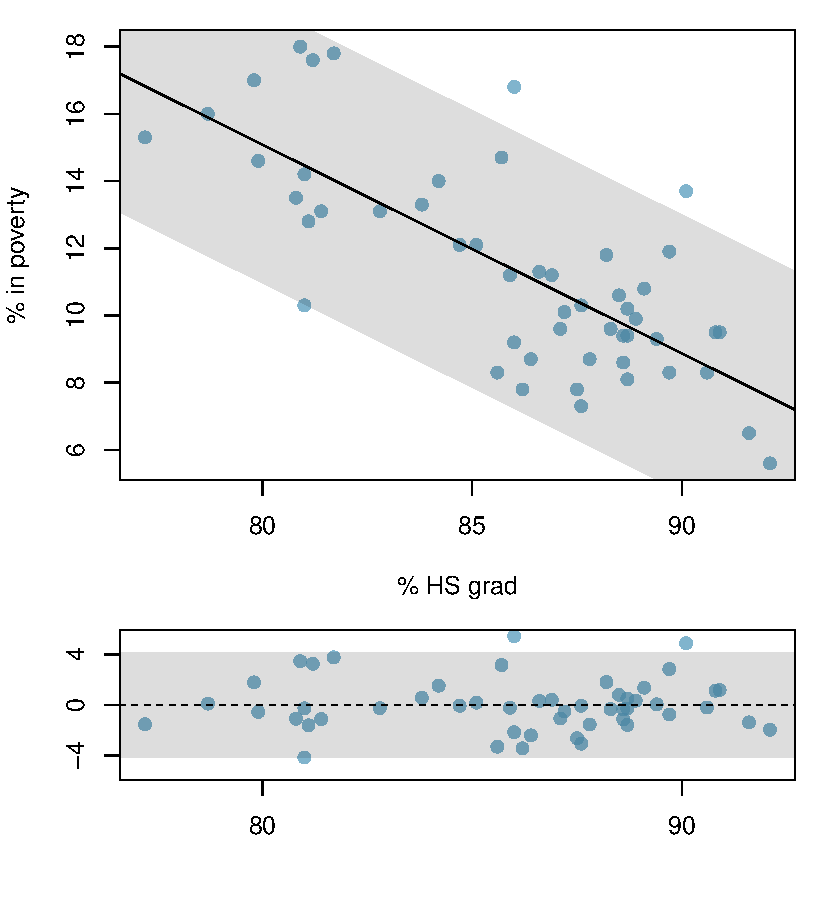
\includegraphics[width=\textwidth]{8-2_least_square_reg/figures/poverty/poverty_hsgrad_tube}
\end{center}
}
{
\begin{itemize}

\item 最小二乗直線の周りの点のばらつきはおおむね一定でなければならない。

\item これは、0の線の周りの残差のばらつきもおおむね一定であることを意味する。

\item \hl{等分散性（homoscedasticity）}とも呼ばれる。

\item 残差プロットを用いて確認する。

\end{itemize}
}


\end{frame}

%%%%%%%%%%%%%%%%%%%%%%%%%%%%%%%%%%

\begin{frame}
\frametitle{条件の確認}

\twocol{0.5}{0.5}
{
\pq{この線形モデルが明らかに違反している条件はどれか？}
\begin{enumerate}[(a)]
\item 等分散性
\solnMult{線形関係}
\item 正規残差
\item 極端な外れ値がない
\end{enumerate}
}
{
\begin{center}
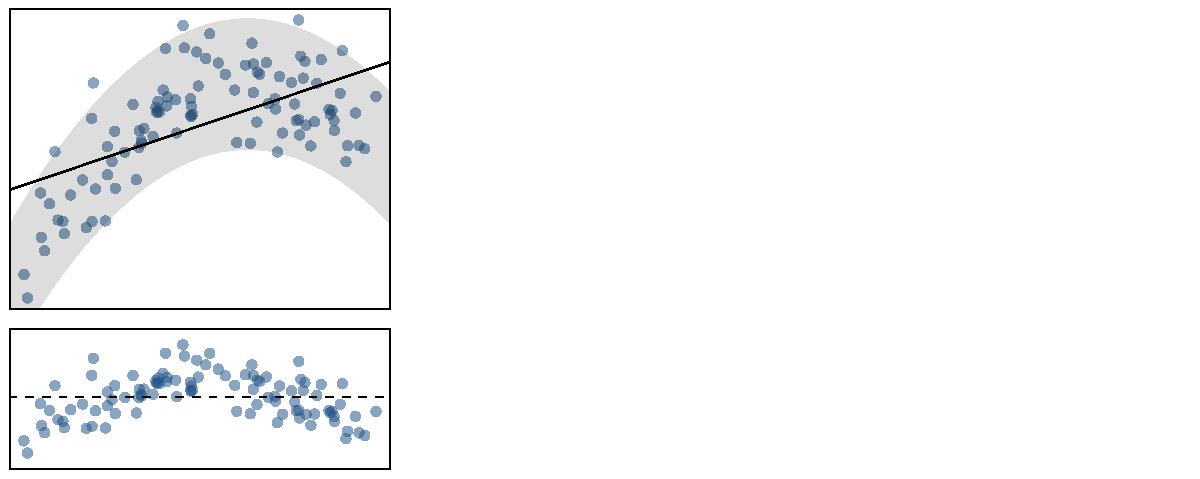
\includegraphics[width=\textwidth]{8-2_least_square_reg/figures/problems/nonlinear}
\end{center}
}

\end{frame}

%%%%%%%%%%%%%%%%%%%%%%%%%%%%%%%%%%

\begin{frame}
\frametitle{条件の確認}

\twocol{0.5}{0.5}
{
\pq{この線形モデルが明らかに違反している条件はどれか？}
\begin{enumerate}[(a)]
\solnMult{等分散性}
\item 線形関係
\item 正規残差
\item 極端な外れ値がない
\end{enumerate}
}
{
\begin{center}
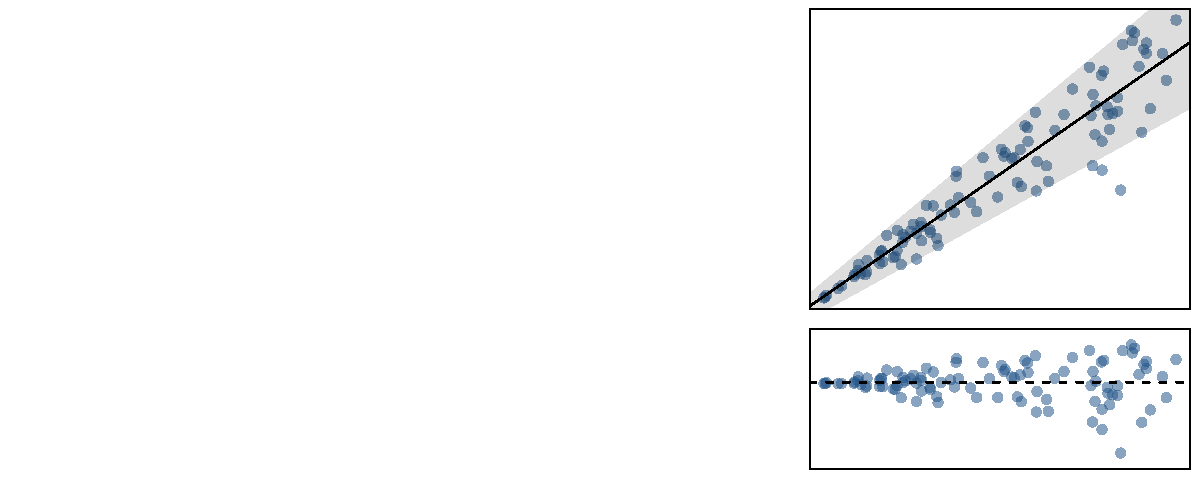
\includegraphics[width=\textwidth]{8-2_least_square_reg/figures/problems/heteroscedastic}
\end{center}
}

\end{frame}

%%%%%%%%%%%%%%%%%%%%%%%%%%%%%%%%%%%

\subsection{最小二乗直線の求め方}

%%%%%%%%%%%%%%%%%%%%%%%%%%%%%%%%%%%

\begin{frame}
\frametitle{与えられたデータ}

\twocol{0.5}{0.5}
{
\begin{center}

\includegraphics[width=0.7\linewidth]{8-2_least_square_reg/figures/poverty/poverty_hsgrad}
\end{center}
}
{
{\scriptsize
\begin{tabular}{l r r}
\hline
		& \shortstack[r]{高校卒業率\\（\%）}	& \shortstack[r]{貧困率\\（\%）} \\
		& $(x)$			& $(y)$ \\
\hline
平均	& $\bar{x} = 86.01$	& $\bar{y} = 11.35$  \\
標準偏差	& $s_x = 3.73$		& $s_y = 3.1$ \\
\hline
		& 相関		& $R = -0.75$ \\
\hline
\end{tabular}
}
}

\end{frame}

%%%%%%%%%%%%%%%%%%%%%%%%%%%%%%%%%%

\subsection{回帰モデルのパラメータ推定値の解釈}

%%%%%%%%%%%%%%%%%%%%%%%%%%%%%%%%%%

\begin{frame}
\frametitle{傾き}

\formula{傾き}
{回帰の傾きは次の式で計算できる：
\[ b_1 = \frac{s_y}{s_x} R \]
}

\hl{具体的には…}
\[ b_1 = \frac{3.1}{3.73} \times (-0.75) = -0.62 \]

$\:$ \\
\hl{解釈} \\
高校卒業率が1\%ポイント上昇するごとに、貧困率は平均的に0.62\%ポイント低下すると予測される。

\end{frame}

%%%%%%%%%%%%%%%%%%%%%%%%%%%%%%%%%%

\begin{frame}
\frametitle{切片}

\formula{切片}
{切片は回帰直線が$y$軸と交わる点である。回帰直線は常に$(\bar{x},\bar{y})$を通るという性質を用いて計算する：
\[ b_0 = \bar{y} - b_1 \bar{x} \]
}

\twocol{0.55}{0.45}
{
\begin{center}
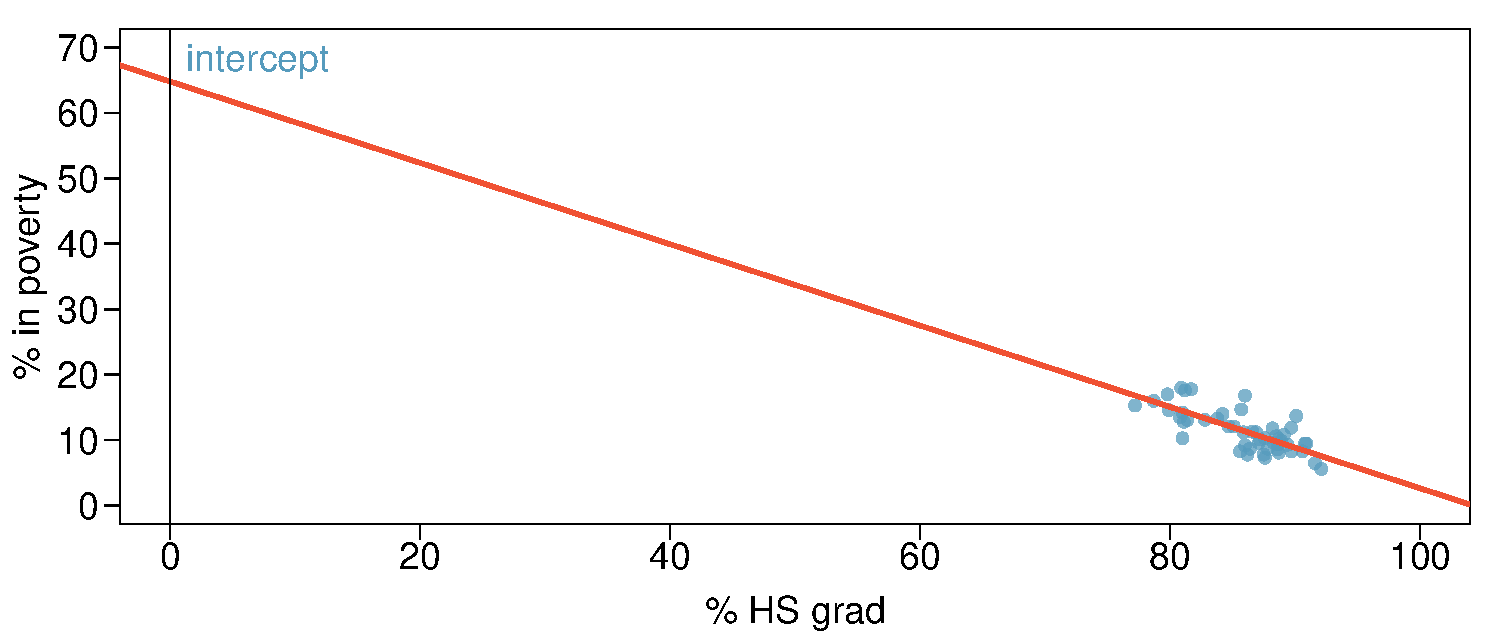
\includegraphics[width=0.75\linewidth]{8-2_least_square_reg/figures/poverty/poverty_hsgrad_line_wide}
\end{center}
}
{
\begin{align*}
b_0 &= 11.35 - (-0.62) \times 86.01 \\
&= 64.68
\end{align*}
}

\end{frame}

%%%%%%%%%%%%%%%%%%%%%%%%%%%%%%%%%%

\begin{frame}
\frametitle{}

\pq{切片の正しい解釈はどれか？}

\begin{enumerate}[(a)]
\item 高校卒業率が1\%ポイント上昇するごとに、貧困率は平均的に64.68\%増加すると予測される。
\item 高校卒業率が1\%ポイント低下するごとに、貧困率は平均的に64.68\%増加すると予測される。
\item 高校卒業者がいない場合、住民の64.68\%が貧困ライン以下で生活する。
\solnMult{高校卒業者がいない州では、住民の平均64.68\%が貧困ライン以下で生活すると予測される。}
\item 高校卒業者がいない州では、貧困率は平均的に64.68\%増加すると予測される。
\end{enumerate}

\end{frame}

%%%%%%%%%%%%%%%%%%%%%%%%%%%%%%%%%%%

\begin{frame}
\frametitle{切片についての補足}

データセットには高校卒業者が一人もいない州は存在しないため、切片はあまり意味を持たず、有用でもなく、切片の予測値がデータの大部分から大きく離れているため信頼性も低い。

\begin{center}
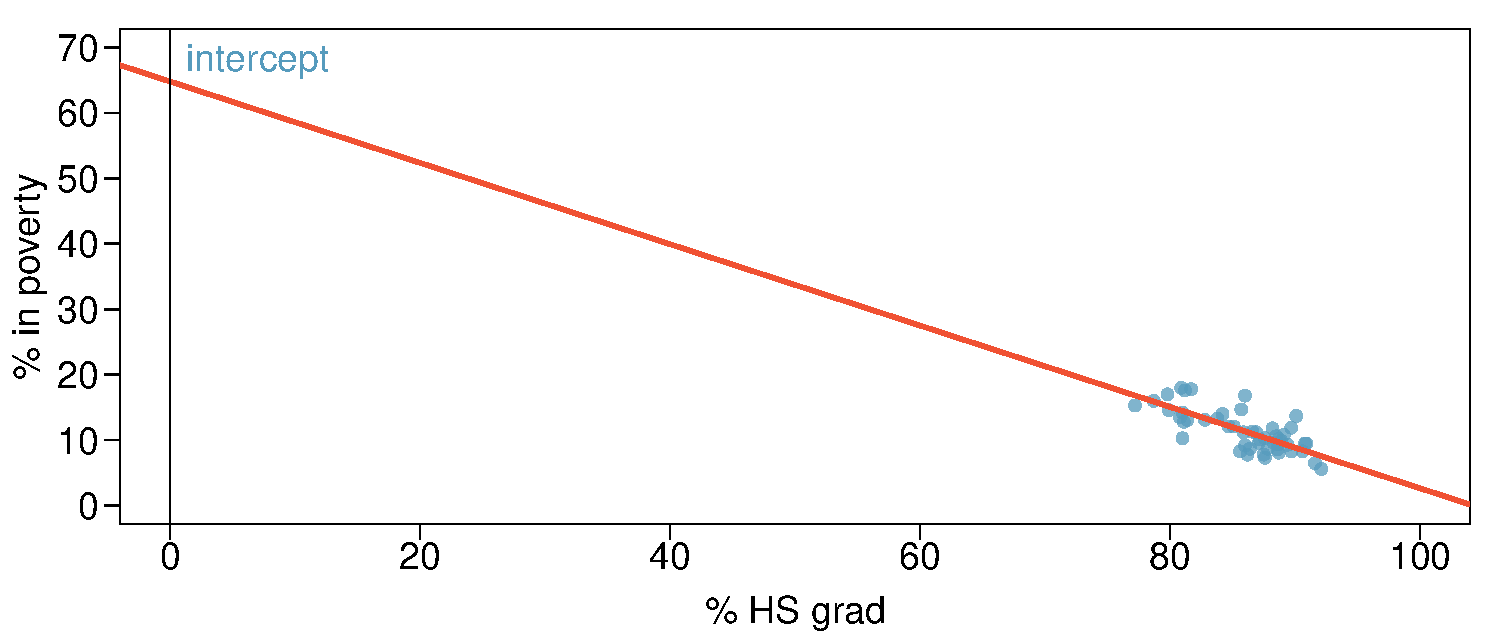
\includegraphics[width=\textwidth]{8-2_least_square_reg/figures/poverty/poverty_hsgrad_line_wide}
\end{center}

\end{frame}

%%%%%%%%%%%%%%%%%%%%%%%%%%%%%%%%%%

\begin{frame}
\frametitle{回帰直線}

\[ \widehat{\%~in~poverty} = 64.68 - 0.62~\%~HS~grad \]

\begin{center}

\includegraphics[width=0.7\textwidth]{8-2_least_square_reg/figures/poverty/poverty_hsgrad_line}
\end{center}

\end{frame}

%%%%%%%%%%%%%%%%%%%%%%%%%%%%%%%%%%

\subsection{まとめ：傾きと切片の解釈}

%%%%%%%%%%%%%%%%%%%%%%%%%%%%%%%%%%%

\begin{frame}
\frametitle{傾きと切片の解釈}

\twocol{0.5}{0.5}{
\begin{itemize}

\item \hl{切片：} $x = 0$のとき、$y$は切片に等しいと予測される。\\

$\:$ \\

\item \hl{傾き：} $x$が1単位増加するごとに、$y$は平均的に傾きの分だけ増加／減少すると予測される。

\end{itemize}
}
{
\begin{center}
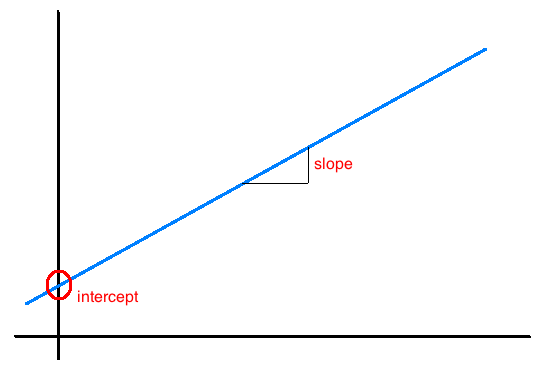
\includegraphics[width=\textwidth]{8-2_least_square_reg/figures/diagram}
\end{center}
}

\vspace{1cm}

\Note{これらの記述は、研究が無作為化比較実験でない限り、因果関係を意味しない。}

\end{frame}


%%%%%%%%%%%%%%%%%%%%%%%%%%%%%%%%%%

\subsection{予測と外挿}

%%%%%%%%%%%%%%%%%%%%%%%%%%%%%%%%%%


\begin{frame}
\frametitle{予測}

\begin{itemize}

\item 線形モデルを用いて、説明変数の特定の値に対する目的変数の値を予測することを\hl{予測}と呼ぶ。線形モデルの式に$x$の値を代入するだけでよい。

\item 予測値には不確かさが伴う。

\end{itemize}

\begin{center}
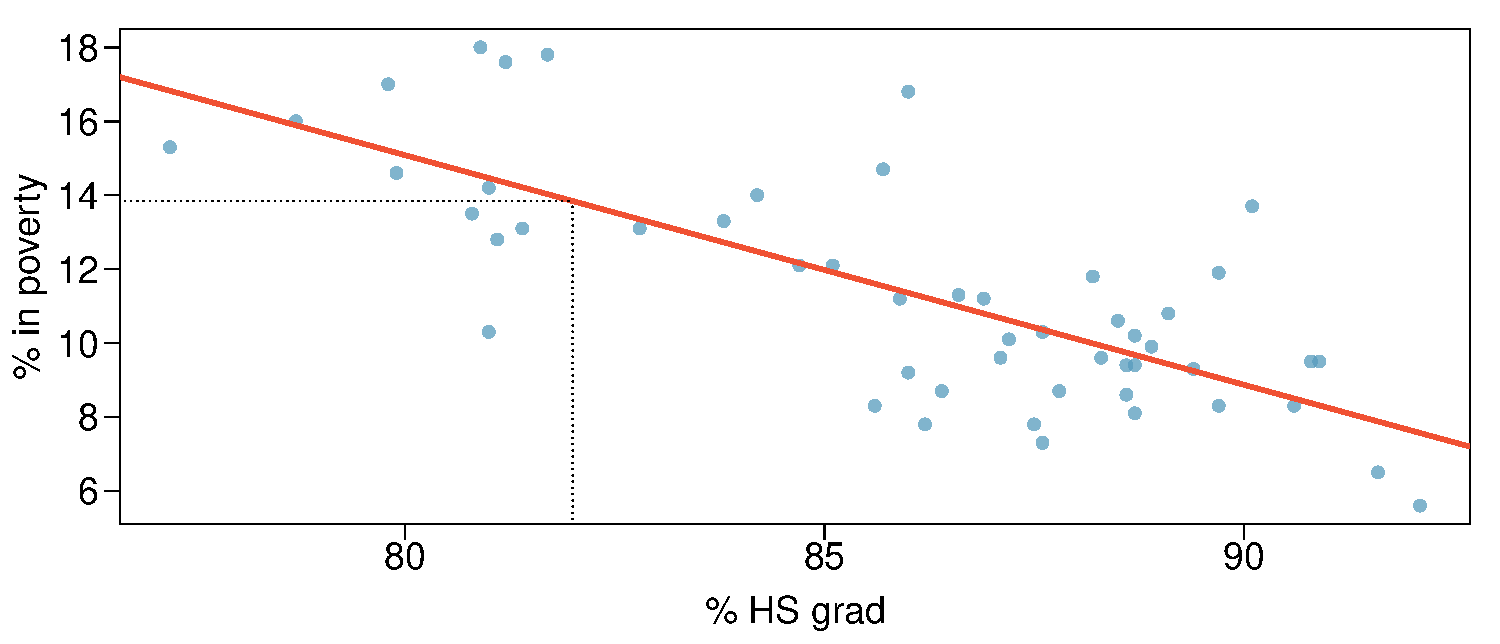
\includegraphics[width=0.9\textwidth]{8-2_least_square_reg/figures/poverty/poverty_hsgrad_pred}
\end{center}

\end{frame}

%%%%%%%%%%%%%%%%%%%%%%%%%%%%%%%%%%

\begin{frame}
\frametitle{外挿}

\begin{itemize}

\item モデルの推定を元のデータの範囲外の値に適用することを\hl{外挿}と呼ぶ。

\item 切片が外挿になる場合もある。

\end{itemize}

\begin{center}
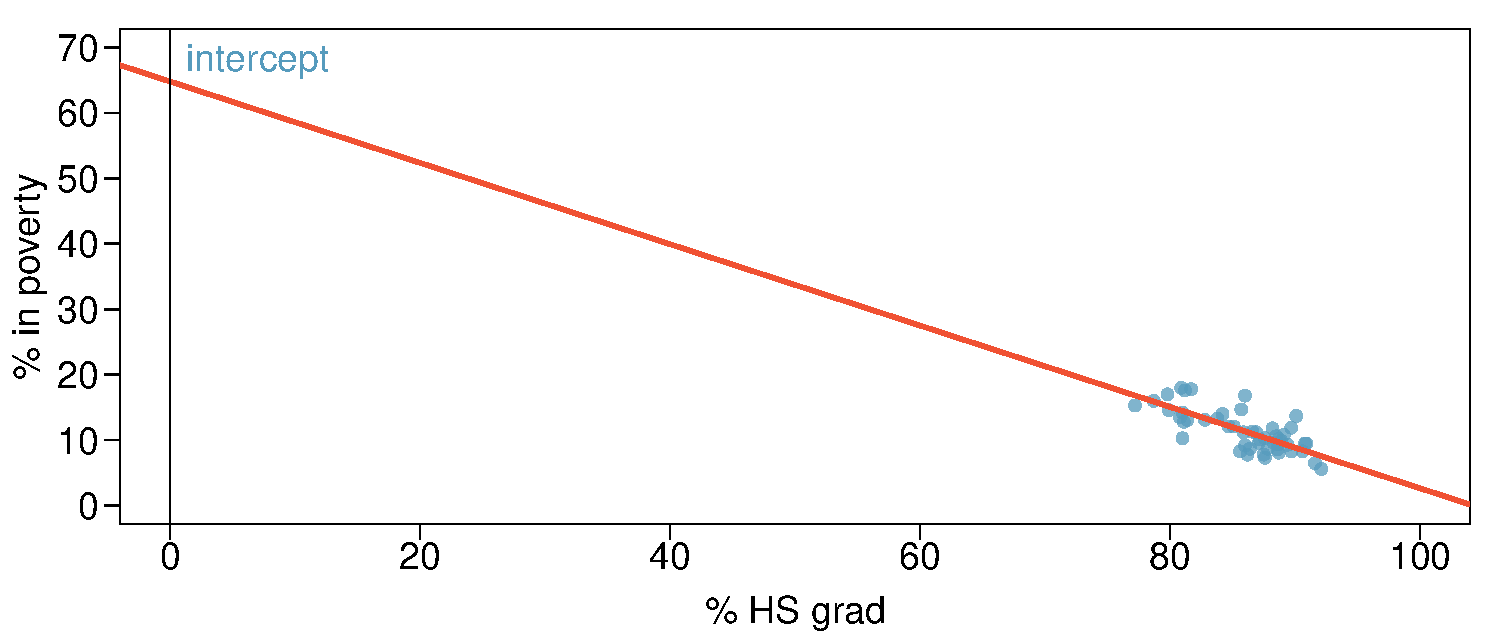
\includegraphics[width=\textwidth]{8-2_least_square_reg/figures/poverty/poverty_hsgrad_line_wide}
\end{center}

\end{frame}

%%%%%%%%%%%%%%%%%%%%%%%%%%%%%%%%%%

\begin{frame}
\frametitle{外挿の例}

\begin{center}
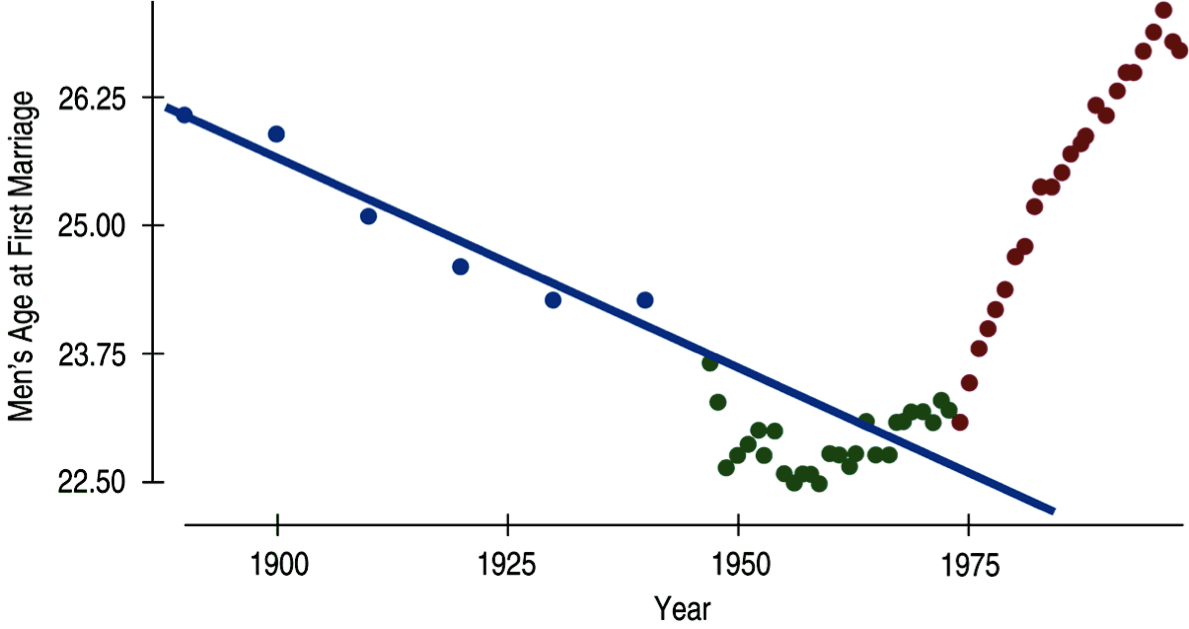
\includegraphics[width=\textwidth]{8-2_least_square_reg/figures/extrapolation}
\end{center}

\end{frame}

%%%%%%%%%%%%%%%%%%%%%%%%%%%%%%%%%%

\begin{frame}
\frametitle{外挿の例}

\begin{center}
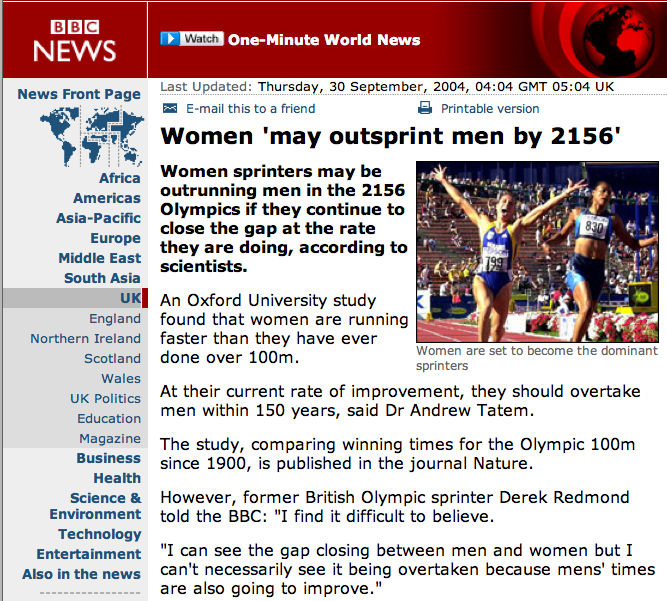
\includegraphics[width=0.7\textwidth]{8-2_least_square_reg/figures/womenOutsprintBBC}
\end{center}

\end{frame}

%%%%%%%%%%%%%%%%%%%%%%%%%%%%%%%%%%

\begin{frame}
\frametitle{外挿の例}

\begin{center}
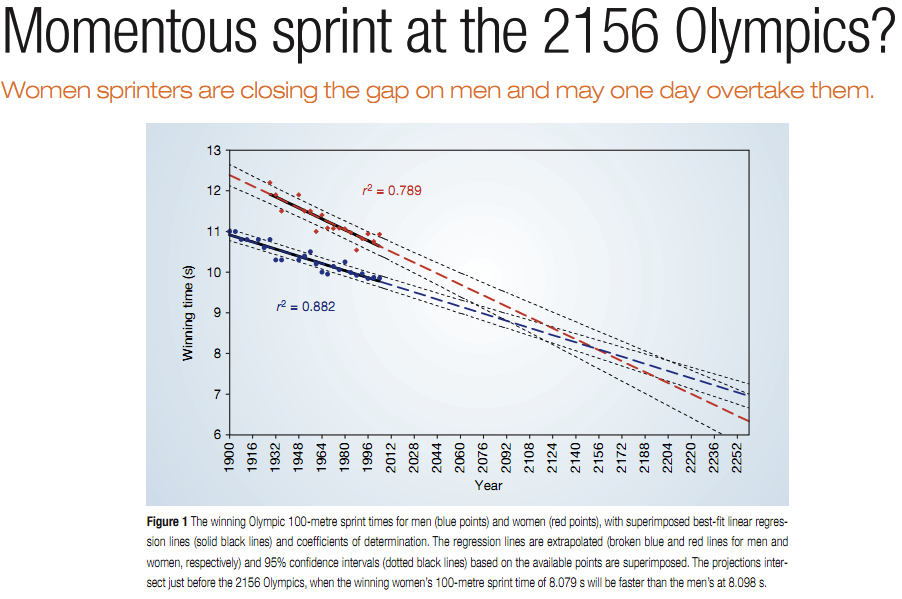
\includegraphics[width=\textwidth]{8-2_least_square_reg/figures/womenOutsprint}
\end{center}

\end{frame}

%%%%%%%%%%%%%%%%%%%%%%%%%%%%%%%%%%

\subsection{$R^2$による当てはまりの強さの記述}

%%%%%%%%%%%%%%%%%%%%%%%%%%%%%%%%%%%

\begin{frame}
\frametitle{決定係数$R^2$}

\begin{itemize}

\item 線形モデルの当てはまりの強さは、通常\mathhl{R^2}（決定係数）を用いて評価する。

\item $R^2$は相関係数の二乗として計算される。

\item 目的変数のばらつきのうち、モデルで説明できる割合を示す。

\item 残りのばらつきは、モデルに含まれていない変数またはデータの固有のランダム性によって説明される。

\item ここで扱っているモデルでは、$R^2 = (-0.75)^2 = 0.56$である。

\end{itemize}

\end{frame}

%%%%%%%%%%%%%%%%%%%%%%%%%%%%%%%%%%

\begin{frame}
\frametitle{$R^2$の解釈}

\pq{{\small $R = -0.75$、$R^2 = 0.56$の正しい解釈はどれか？}}

\twocol{0.65}{0.35}{
\begin{enumerate}[(a)]

\item 51州における高校卒業率のばらつきの56\%はモデルで説明できる。

\solnMult{51州における貧困率のばらつきの56\%はモデルで説明できる。}

\item 高校卒業率が貧困率を正しく予測できる割合は56\%である。

\item 51州における貧困率のばらつきの75\%はモデルで説明できる。

\end{enumerate}
}{
\begin{center}

\includegraphics[width=\textwidth]{8-2_least_square_reg/figures/poverty/poverty_hsgrad}
\end{center}
}

\end{frame}

%%%%%%%%%%%%%%%%%%%%%%%%%%%%%%%%%%
